\subsection{Fonctionnement}
Contrairement aux compteurs électro-mécaniques qui doivent être relevés manuellement, les compteurs intelligents :

\begin{itemize}[label=\textbullet]
\item Enregistrent dans leur mémoire, selon un protocole défini, la puissance électrique prélevée et les quantités consommées à différents moments de la journée chaque jour de la semaine.
\item Transmettent de manière électronique ces données au gestionnaire de réseau  ou au client.
\item Peuvent être contrôlés et vérifiés à distance par le gestionnaire de réseau.
\item Envoient une alarme au gestionnaire de réseau en cas d’ouverture du capot et donc, de suspicion de fraude.
\end{itemize}

\begin{figure}[h]
	\centering
    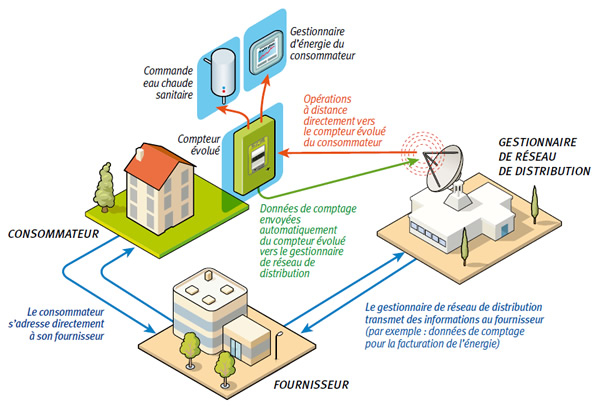
\includegraphics[scale=0.6]{img/part2/1.5}
    \caption{Fonctionnement du compteur intelligent}
\end{figure}